\documentclass[12pt]{article}
\def\x#1#2{$\mathbb{#1}^#2$} 
\def\n#1{\x#1}

\usepackage{graphicx}
\usepackage{latexsym}
\usepackage{amsfonts}
\usepackage{listings}
\usepackage{mypriptrt}
\usepackage{subfigure}
\usepackage{epic}


\title{NC LU - Abgabe 1} 
\author{Aidoma, Kern, Weichselbaum}

\abstract{
	Documentation for the first exercise of Neural Computation LU, Group 8.
}
\begin{document}
	
\maketitle	
	

\section{Introduction}

The exercises are split up into several files. However, for convenience purposes all exercises can be executed by the function ex in the m-file named 'ex.m'.

\section{Exercise 1.1}
\subsection{Exercise 1.1.1}
\textit{Stellen Sie die Lage der Datenvektoren und ihre labels graphisch dar.}

\begin{figure}[htp]
	\centering
	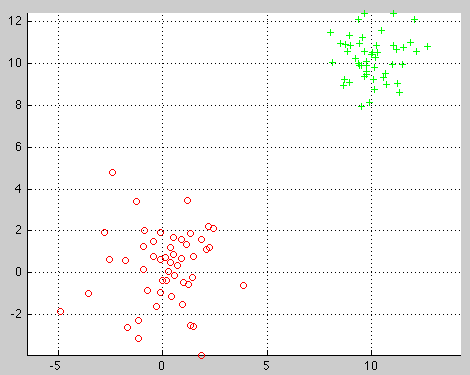
\includegraphics[width=1\textwidth]{ab1_1_1.png}
	\caption{Dataset generated with genData(50,2)}
	\label{fig:vector}
\end{figure}

\subsection{Exercise 1.1.2}

\textit{Untersuchen sie den Trainingsalgorithmus: Wieviele Iterationen werden benoetigt, bis sich weight-Vektor $w$ im Fall von linear separierbaren Daten nicht mehr andert?}
\\
It takes 9 epochs until the weight vector doesn't change. At this point, the algorithm stops because all of the data entries are successfully classified.
\\
\\
\textit{Wie veraendert sich der w waehrend des Trainings?}
\\
The weight vector is changed at each iteration IFF the data entry is misclassified. If it is misclassified the product of gamma, data entry and target for the data entry is added to the current weight vector.
\\
\\

\textit{Welchen Einfluss hat die Schrittweite?}
\\
The step width, gamma, did not significantly influence the numbers of epochs needed. On our randomly generated dataset we trained our perceptron with different gammas from 0.01 to 1, gradially increasing it by the value of 0.01 and stored the
resulting number of epochs needed, each run. To acquire enough testdata we repeated this test with different randomly generated datasets 100 times. When performing a correlation test on the resulting pairs of data, its result leads to the conclusion
that gamma doesn't correlate with the needed number of adjustments of the weight vector.\\
The dataset has been created with gendata(100,2) and the resulting correlation coefficient between gamma and epoch number, was -0.0095. 
\\
\\


\textit{Plotten Sie die Daten und Entscheidungsgrenze in \n{R2}}
\\
Shown in Figure \ref{fig:entscheidung}
\\
\begin{figure}[htp]
	\centering
	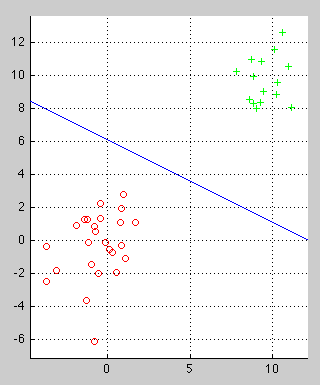
\includegraphics[width=1\textwidth]{ab1_1_2.png}
	\caption{Daten mit Entscheidungsgrenze (Split 90\%) }
	\label{fig:entscheidung}
\end{figure}
\\
\\

\textit{Wie ist das Verhalten bei nicht linear separierbaren Daten?}
\\
Unfortunately, the algorithm runs until maxIts (variable setting the maximum of possible epochs) is reached. Since the data is not linearly seperable there will always be a data entry on the wrong side of the hyperplane and therefor rotating it will not result in a success. The algorithm would run indefinitely without maxIts. 

\subsection{Exercise 1.1.3}
\textit{Untersuchen Sie die Leistung des trainierten Perzeptrons auf dem Testset abhaengig von der Groesse des Trainingsets.}
\\
\begin{figure}[htp]
	\centering
	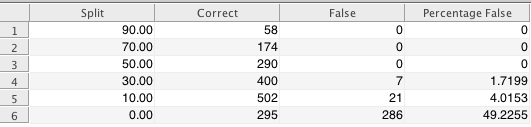
\includegraphics[width=0.8\textwidth]{ab1_1_3}
	\caption{Our randomly generated dataset, genData(50,2)}
	\label{fig:diff}
\end{figure}
\\
Figure \ref{fig:diff} shows the differences in 20\% split steps.
\\

\textit{Stellen Sie fuer einen Vergleich die wahren und die vom Perzeptron generierten Datenlabels graphisch dar.}
\\
This is answered/shown in 1.1.3.

\section{Exercise 1.2}
\subsection{Exercise 1.2.1}

Figure \ref{fig:dataQuadReg} plots the function $y=2x^2 - 8x + 1$. The plotted points is the data used for regression in next section.

\begin{figure}[htp]
	\centering
	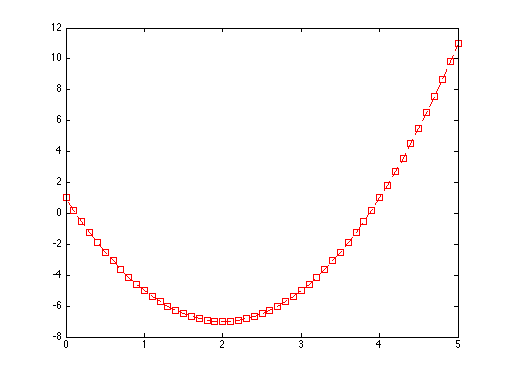
\includegraphics[width=0.8\textwidth]{ab1_2_1.png}
	\caption{Generated data for quadratic regression}
	\label{fig:dataQuadReg}
\end{figure}

\subsection{Exercise 1.2.2}
\textit{Wieviele und welche basis functions $\Phi_i$ verwenden Sie? }\\

In this case we are using three basis functions listed below:
\begin{itemize}
\item $\Phi_0=1$
\item $\Phi_1=x$
\item $\Phi_2=x^2$
\end{itemize}
\textit{Welche cost function ergibt sich?}

The cost function we are minimizing in linear regression is the SSE:
\begin{equation}E(w, x_i) = \frac{1}{2}\sum_{i=1}^N(t_i - w_i\Phi_i(x_i))^2\end{equation} \\
\textit{Untersuchen Sie den Einfluss der Schrittweite $\gamma$ auf das Konvergenzverhalten.}\\
\textit{ Welches $\gamma$ ergibt eine guten tradeoff zwischen Trainingszeit und Konvergenz- 
verhalten? Gibt es ein  $\gamma$, bei dem $w$ divergiert}\\
\textit{Wieviele Epochen benoetigt der Algorithmus?}\\

All three questions are answered together because of the direct relationship between convergence and step $\gamma$. By fixing the number of epochs,
we can inspect the cost function according to the desired step $\gamma$ used. The other way round, we can fix a desired
error to inspect the number of epochs for a fixed step $\gamma$. When the desired value of the cost function is reached, then the algorithm must stop. 

In table \ref{table:gammaSSE} we show the results of the experiments. The algorithm will stop if the value of the cost function is lower than 0.0001 or the maximum
number of iterations is reached. In this case, $1000$ iterations. Epoch values of $-1$ means that the algorithm used the maximum number of iterations without reaching the desired value for the cost function.\\\\

As we can see in table \ref{table:gammaSSE}, for values of $\gamma$ bigger than $0.012$ the algorithm does not converge. Obviously, the step giving the best trade-off is the higher $\gamma$ where the algorithm still converges, so $0.012$.
      
\begin{table}
\centering
\begin{tabular}{rll} 
  \hline
  $\gamma$ & $E(w,X)$ & Epochs \\
  \hline \hline
  0.001 & 0.131765447252177 & -1 \\
  \hline
  0.003 & $<0.0001$ & 889 \\
  \hline
  0.005 & $<0.0001$ & 608 \\
  \hline
  0.007 & $<0.0001$ & 477 \\
  \hline
  0.009 & $<0.0001$ & 400 \\
  \hline
  0.011 & $<0.0001$ & 361 \\
  \hline
   0.013 & Inf & -1 \\
  \hline
\end{tabular}
\label{table:gammaSSE}
\caption{$E(w,X)$ for different $\gamma$}
\end{table}\end{document}


